\documentclass[10pt]{beamer}
\usepackage{uglixbeamer}
\usepackage{animate}
\title{CH13 : \\Files}
\author{T$^{\text{ale}}$ NSI}
\begin{document}
	\maketitle

\begin{frame}{Principe}
\only<1>{\begin{center}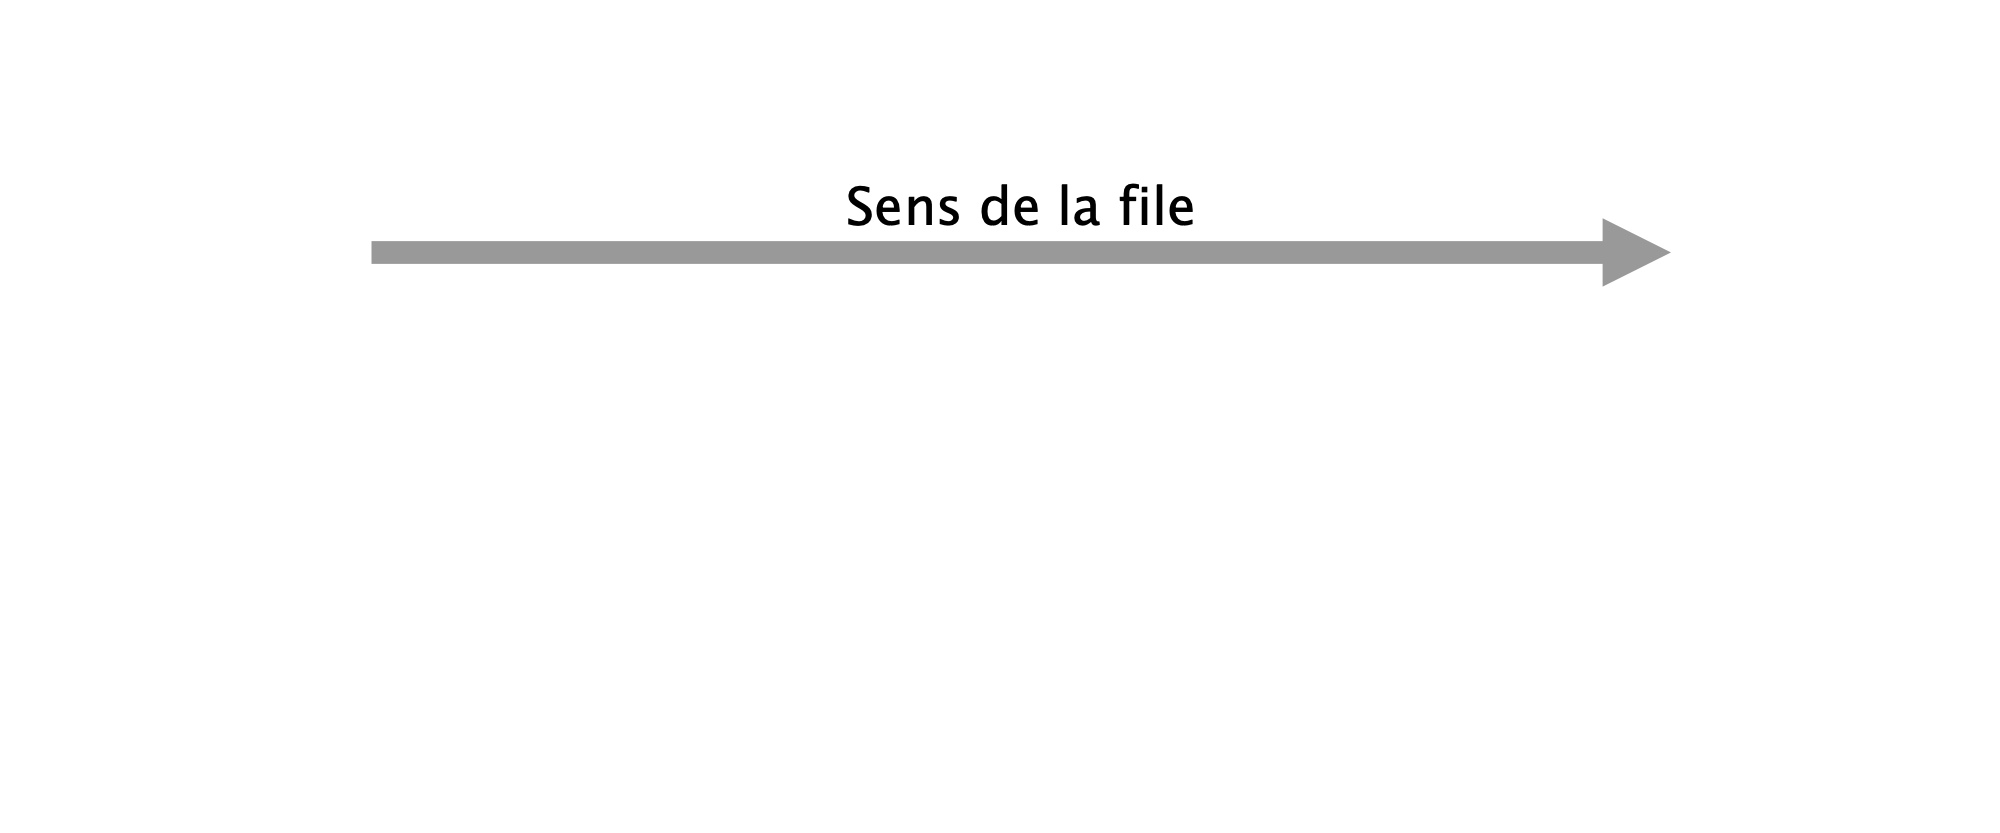
\includegraphics[width=8cm]{img/file0}\\ On part d'une file vide.\end{center}}
\only<2>{\begin{center}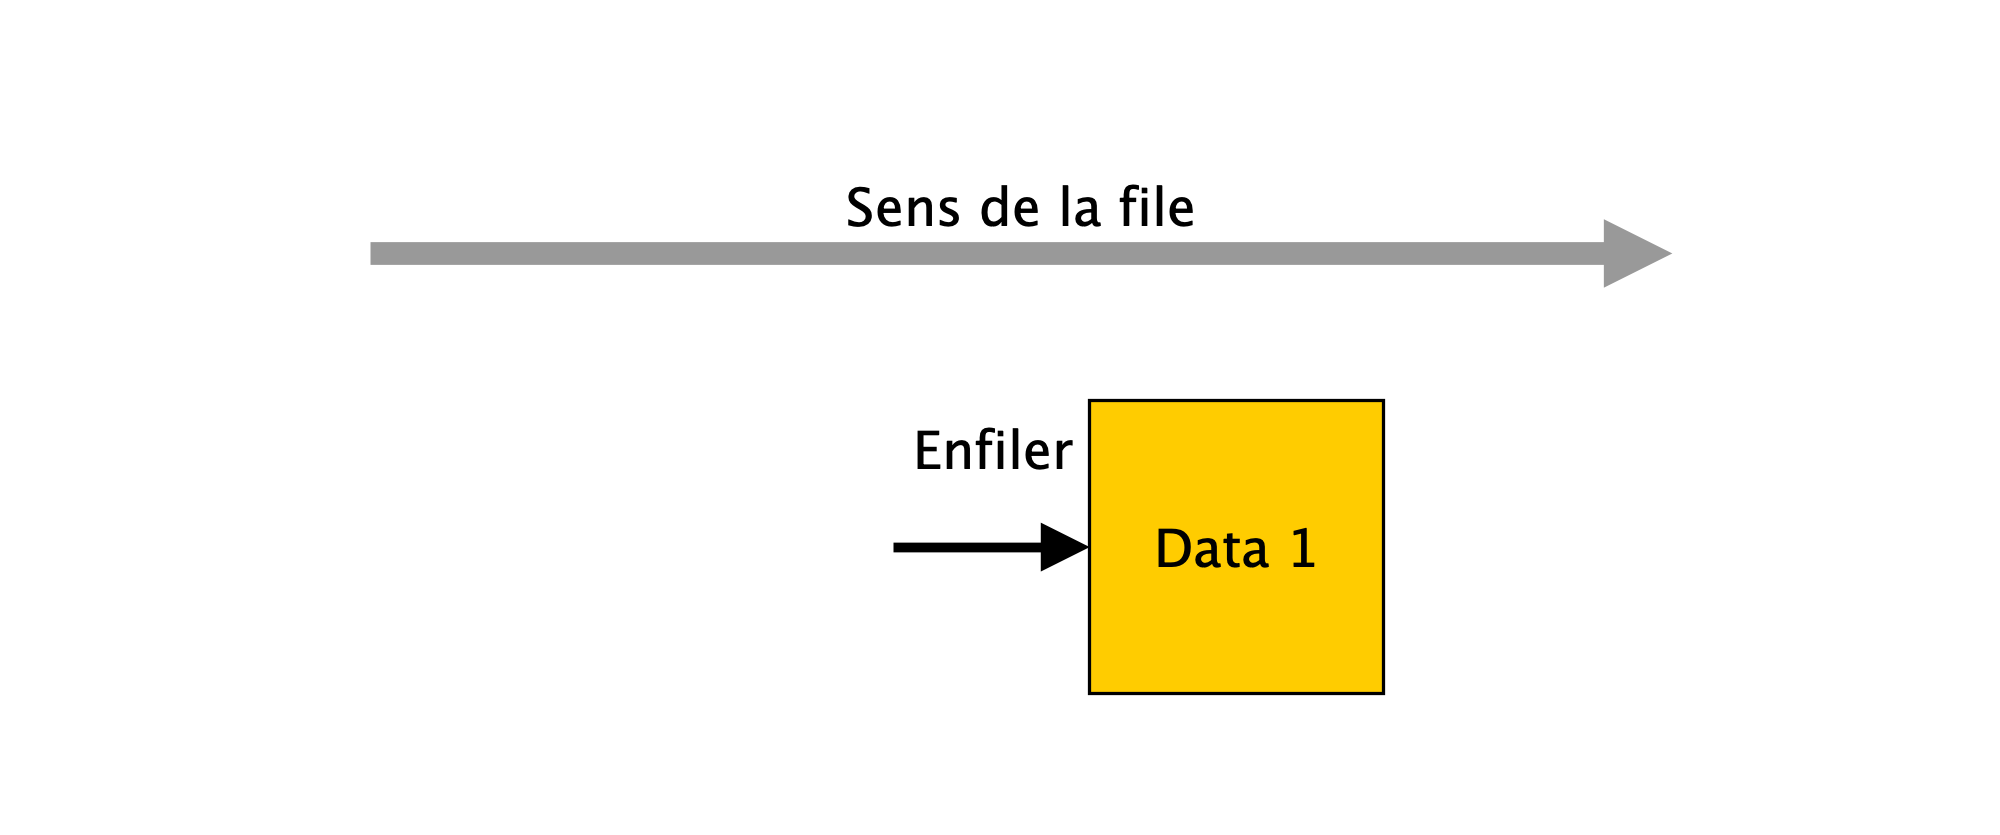
\includegraphics[width=8cm]{img/file1}\\ On enfile les éléments...\end{center}}
\only<3>{\begin{center}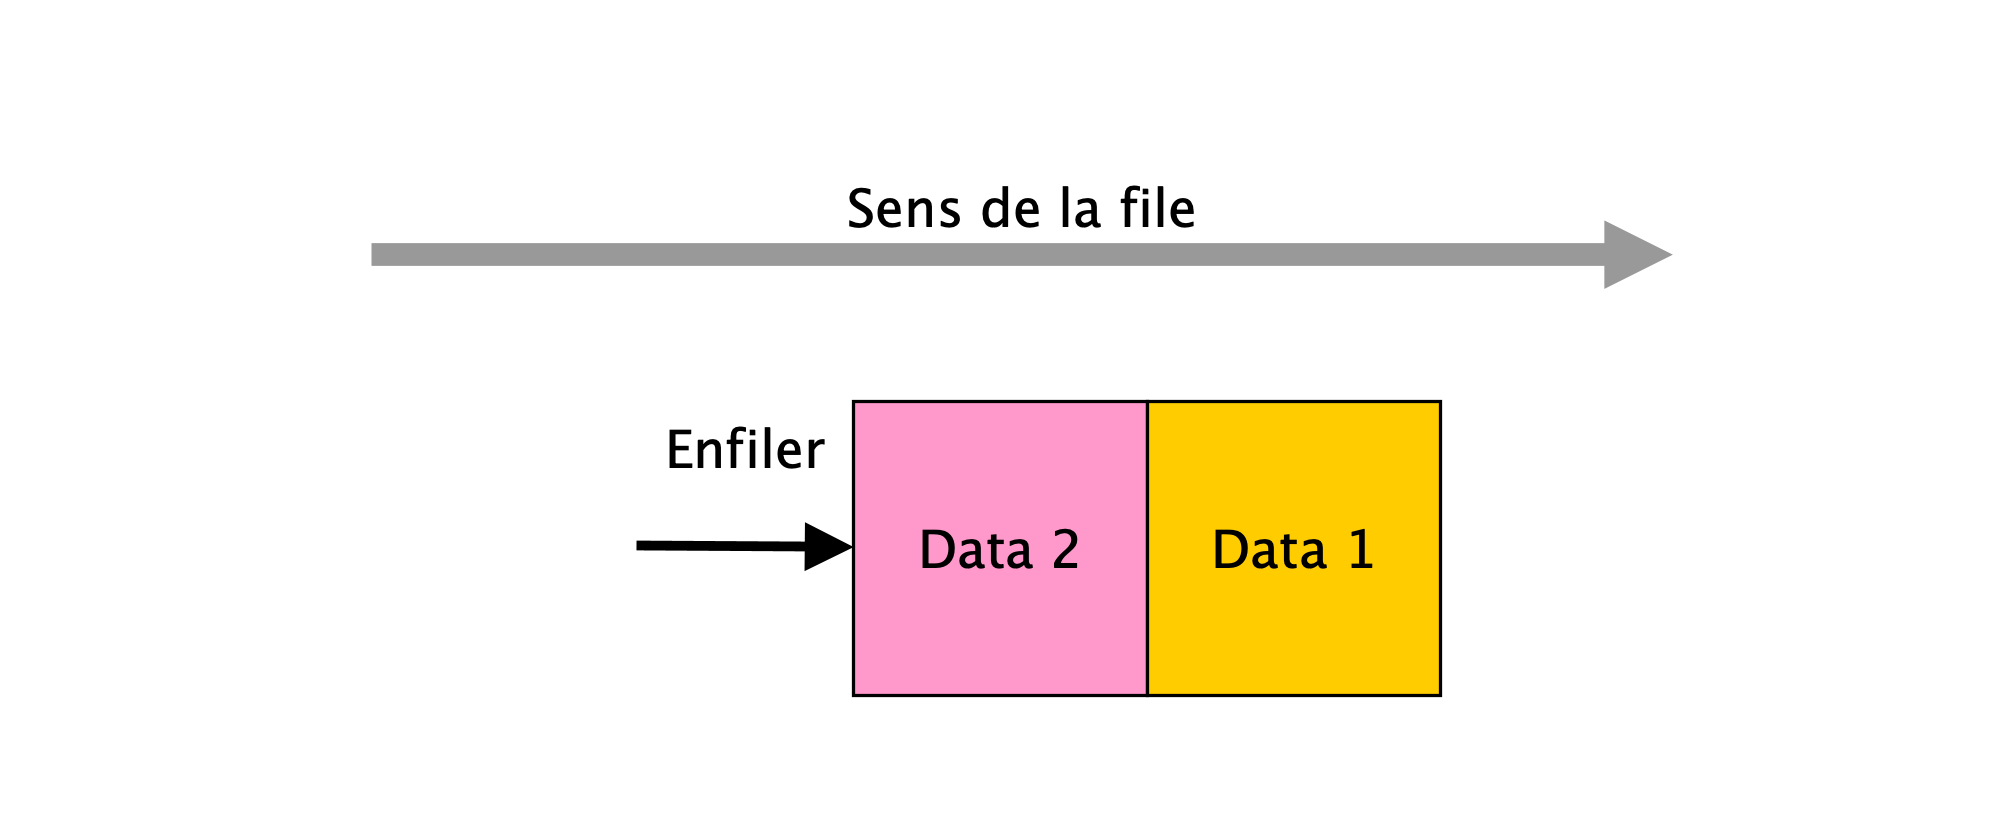
\includegraphics[width=8cm]{img/file2}\\ ... un par un.\end{center}}
\only<4>{\begin{center}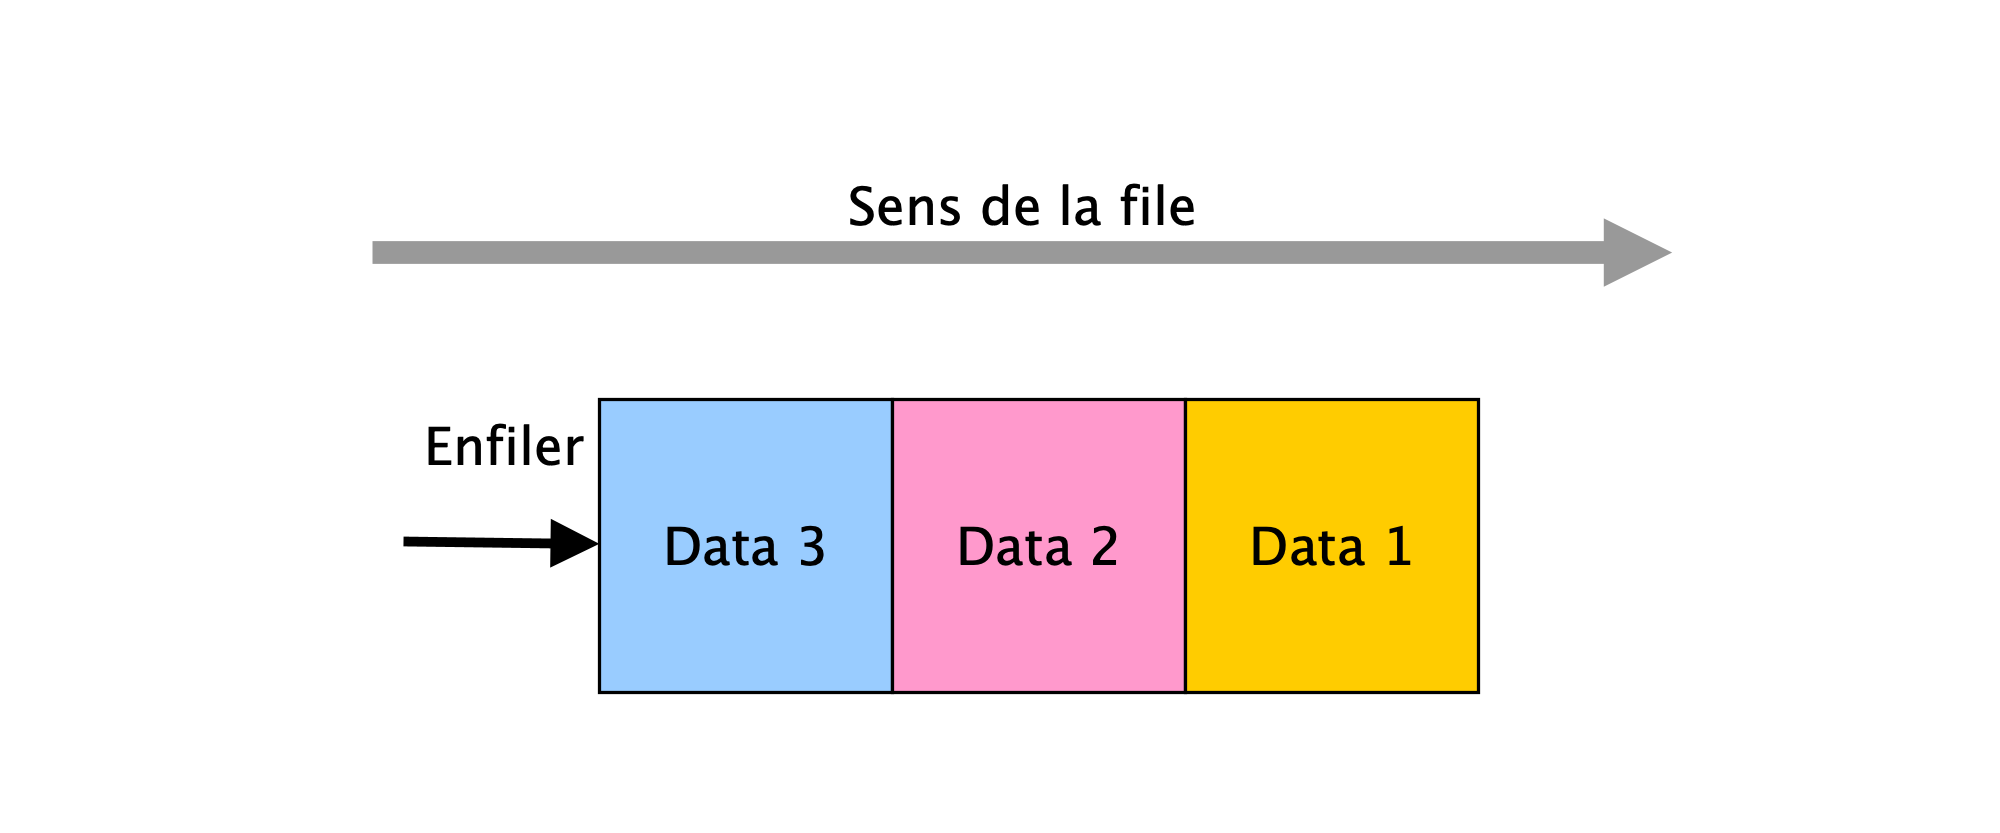
\includegraphics[width=8cm]{img/file3}\end{center}}
\only<5>{\begin{center}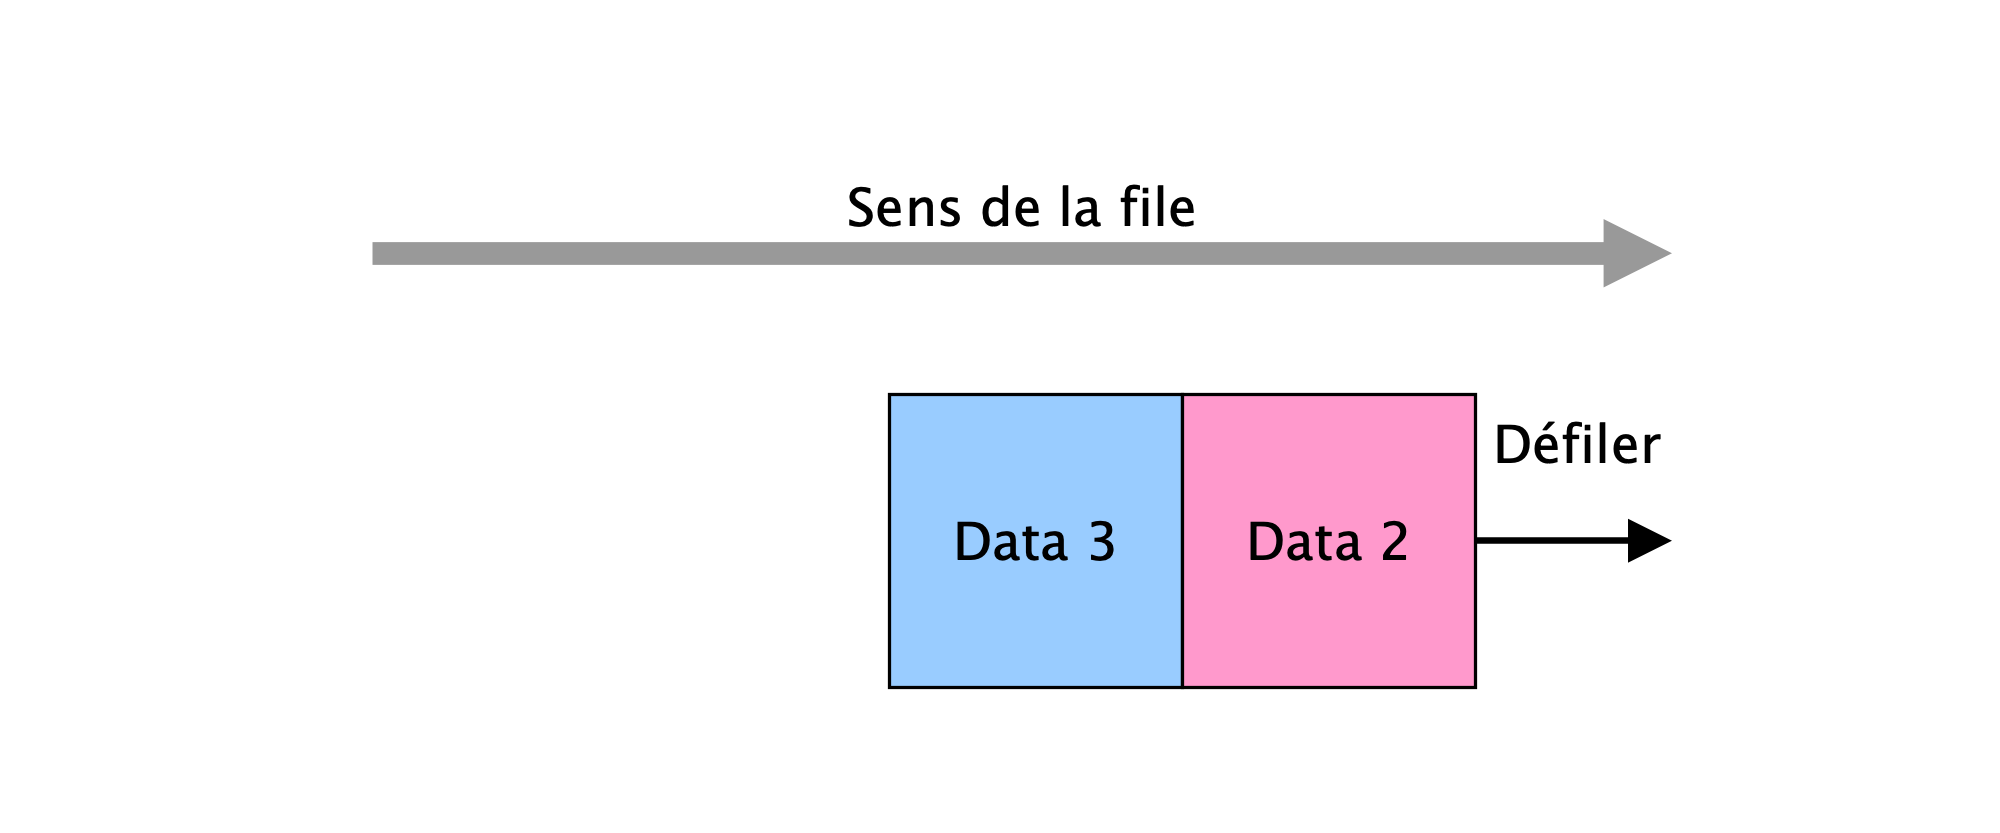
\includegraphics[width=8cm]{img/file4}\\ On ne peut que retirer le premier élément enfilé.\end{center}}
\only<6>{\begin{center}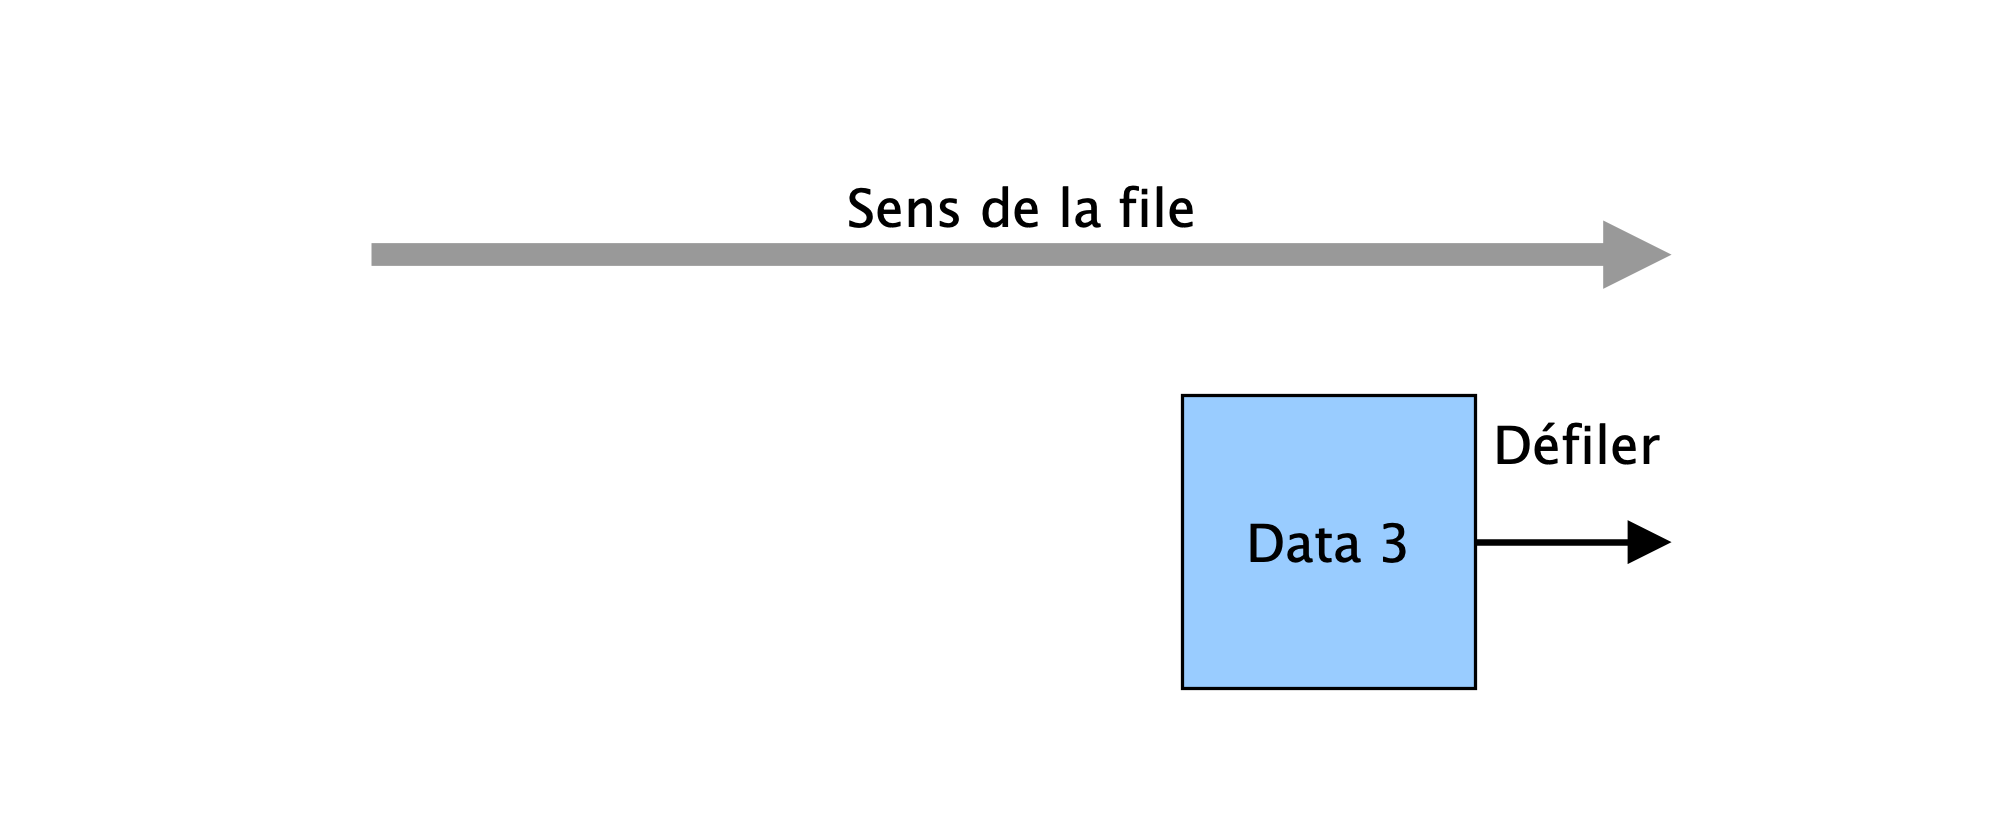
\includegraphics[width=8cm]{img/file5}\\ \og Premier entré, premier sorti\fg{} : \textit{First in first out} (FIFO).\end{center}}				
\end{frame}
\begin{frame}{Applications}
	\begin{itemize}
		\item 	File d'impression de documents.
		\item 	File d'évènements dans \texttt{pygame} ou en général en programmation \textit{évènementielle}.
		\item	Algorithmes de gestion des stocks.
		\item 	Parcours de graphes et d'arbres.
		\item 	D'autres applications sont données en exercice.
	\end{itemize}
\end{frame}
\begin{frame}{Interface de la structure de données file}
	Elle est très simple !
	\begin{itemize}
		\item \textit{file\_vide()} créée une file vide
		\item \textit{enfiler(pile,valeur)} enfile la valeur dans la file
		\item  \textit{defiler(pile)} renvoie le prochain élément dans la file et l'enlève
		\item \textit{est\_vide()} indique si la file est vide on non	 
	\end{itemize}
\end{frame}
\begin{frame}{Implémentations}
	\begin{itemize}
		\item Avec une simple liste python.
		\item Avec une liste encapsulée dans un objet.
		\item Avec 2 piles !
	\end{itemize}
\end{frame}
\begin{frame}{Fabriquer une file avec 2 piles}
    \begin{center}
	\animategraphics[loop,autoplay,width=6cm]{0.8}{img/2piles1file/f}{00}{20}
    \end{center}
\end{frame}
\end{document}